\documentclass[tikz,border=8pt]{standalone}
% Shared look for every TikZ diagram. Load with % Shared look for every TikZ diagram. Load with % Shared look for every TikZ diagram. Load with \input{../../tools/tikz-style.tex}
\usepackage[T1]{fontenc}
\usepackage{lmodern}
\renewcommand{\sfdefault}{lmr}  % diagrams use the same serif as the text
\usetikzlibrary{arrows.meta, positioning, shapes.geometric, calc, fit, backgrounds}
\definecolor{cblue}{HTML}{4C78A8}
\definecolor{corange}{HTML}{F58518}
\definecolor{cgreen}{HTML}{54A24B}
\definecolor{cred}{HTML}{E45756}
\definecolor{cpurple}{HTML}{B279A2}
\definecolor{cgrey}{HTML}{6B6B6B}
\tikzset{
  every picture/.style={font=\sffamily, line width=1.2pt},
  box/.style={draw=#1, fill=#1!12, rounded corners=4pt, align=center, inner sep=7pt, minimum height=1.1cm},
  box/.default=cgrey,
  arrow/.style={-{Stealth[length=3mm]}, draw=cgrey, line width=1.4pt},
  title/.style={font=\sffamily\bfseries\Large},
  note/.style={font=\sffamily\small, text=cgrey, align=center},
}
\AtBeginDocument{\hyphenpenalty=10000 \exhyphenpenalty=10000}

\usepackage[T1]{fontenc}
\usepackage{lmodern}
\renewcommand{\sfdefault}{lmr}  % diagrams use the same serif as the text
\usetikzlibrary{arrows.meta, positioning, shapes.geometric, calc, fit, backgrounds}
\definecolor{cblue}{HTML}{4C78A8}
\definecolor{corange}{HTML}{F58518}
\definecolor{cgreen}{HTML}{54A24B}
\definecolor{cred}{HTML}{E45756}
\definecolor{cpurple}{HTML}{B279A2}
\definecolor{cgrey}{HTML}{6B6B6B}
\tikzset{
  every picture/.style={font=\sffamily, line width=1.2pt},
  box/.style={draw=#1, fill=#1!12, rounded corners=4pt, align=center, inner sep=7pt, minimum height=1.1cm},
  box/.default=cgrey,
  arrow/.style={-{Stealth[length=3mm]}, draw=cgrey, line width=1.4pt},
  title/.style={font=\sffamily\bfseries\Large},
  note/.style={font=\sffamily\small, text=cgrey, align=center},
}
\AtBeginDocument{\hyphenpenalty=10000 \exhyphenpenalty=10000}

\usepackage[T1]{fontenc}
\usepackage{lmodern}
\renewcommand{\sfdefault}{lmr}  % diagrams use the same serif as the text
\usetikzlibrary{arrows.meta, positioning, shapes.geometric, calc, fit, backgrounds}
\definecolor{cblue}{HTML}{4C78A8}
\definecolor{corange}{HTML}{F58518}
\definecolor{cgreen}{HTML}{54A24B}
\definecolor{cred}{HTML}{E45756}
\definecolor{cpurple}{HTML}{B279A2}
\definecolor{cgrey}{HTML}{6B6B6B}
\tikzset{
  every picture/.style={font=\sffamily, line width=1.2pt},
  box/.style={draw=#1, fill=#1!12, rounded corners=4pt, align=center, inner sep=7pt, minimum height=1.1cm},
  box/.default=cgrey,
  arrow/.style={-{Stealth[length=3mm]}, draw=cgrey, line width=1.4pt},
  title/.style={font=\sffamily\bfseries\Large},
  note/.style={font=\sffamily\small, text=cgrey, align=center},
}
\AtBeginDocument{\hyphenpenalty=10000 \exhyphenpenalty=10000}

\begin{document}
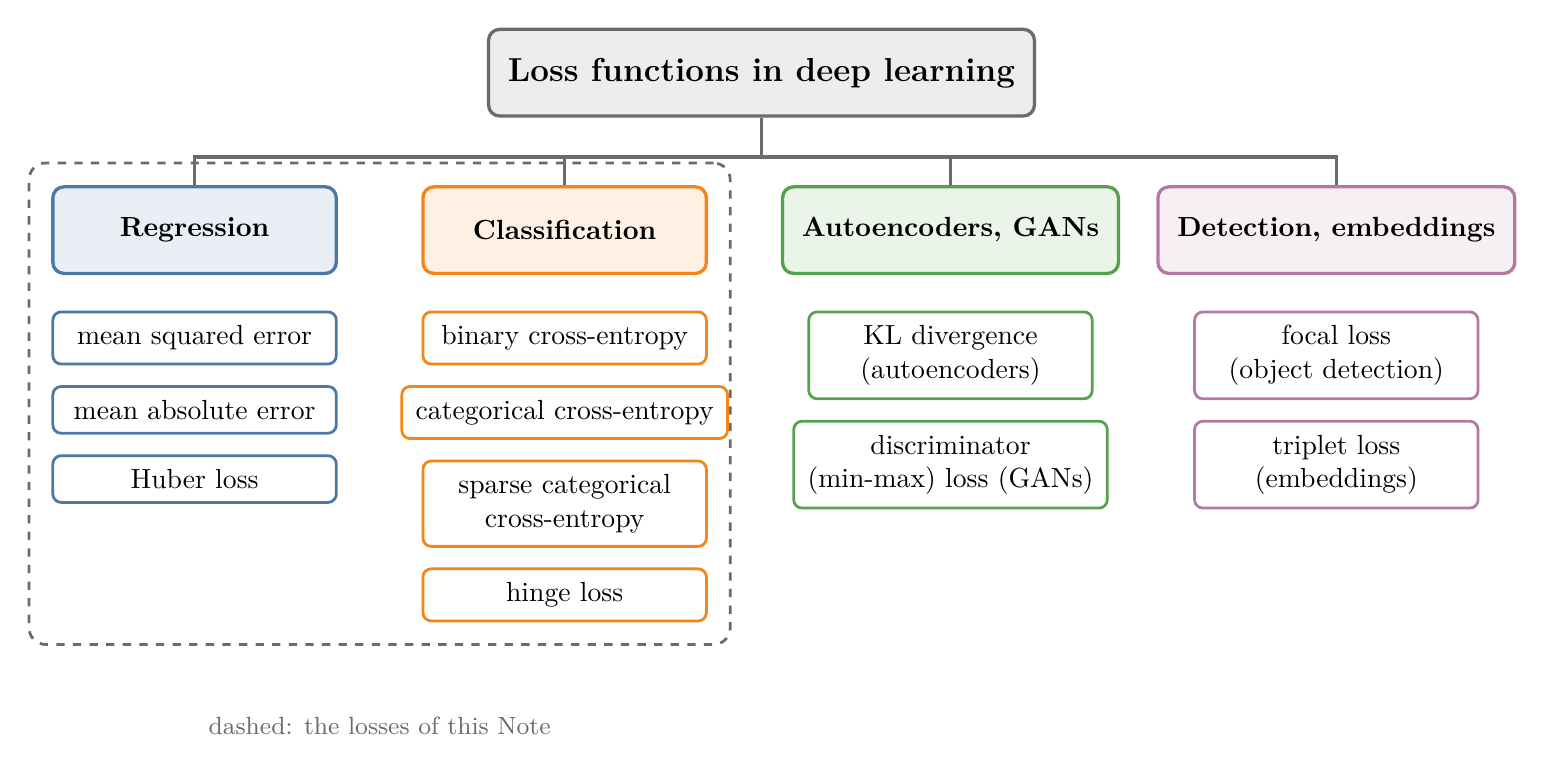
\begin{tikzpicture}[
  root/.style={box=cgrey, font=\sffamily\bfseries\large, minimum width=4.2cm},
  group/.style={box=#1, font=\sffamily\bfseries, minimum width=3.6cm},
  leaf/.style={draw=#1, fill=white, rounded corners=3pt, align=center, inner sep=5pt, minimum width=3.6cm,
               font=\sffamily\normalsize, line width=1pt},
  link/.style={draw=cgrey, line width=1.1pt}]
  \node[root] (r) at (0, 0) {Loss functions in deep learning};
  % four groups
  \node[group=cblue]   (reg) at (-7.2, -2) {Regression};
  \node[group=corange] (cls) at (-2.5, -2) {Classification};
  \node[group=cgreen]  (gen) at ( 2.4, -2) {Autoencoders, GANs};
  \node[group=cpurple] (oth) at ( 7.3, -2) {Detection, embeddings};
  \foreach \g in {reg, cls, gen, oth} \draw[link] (r.south) -- ++(0,-0.5) -| (\g.north);
  % leaves
  \node[leaf=cblue, below=0.45cm of reg] (r1) {mean squared error};
  \node[leaf=cblue, below=0.25cm of r1] (r2) {mean absolute error};
  \node[leaf=cblue, below=0.25cm of r2] (r3) {Huber loss};
  \node[leaf=corange, below=0.45cm of cls] (c1) {binary cross-entropy};
  \node[leaf=corange, below=0.25cm of c1] (c2) {categorical cross-entropy};
  \node[leaf=corange, below=0.25cm of c2] (c3) {sparse categorical\\cross-entropy};
  \node[leaf=corange, below=0.25cm of c3] (c4) {hinge loss};
  \node[leaf=cgreen, below=0.45cm of gen] (g1) {KL divergence\\(autoencoders)};
  \node[leaf=cgreen, below=0.25cm of g1] (g2) {discriminator\\(min-max) loss (GANs)};
  \node[leaf=cpurple, below=0.45cm of oth] (o1) {focal loss\\(object detection)};
  \node[leaf=cpurple, below=0.25cm of o1] (o2) {triplet loss\\(embeddings)};
  \node[note] at (-4.85, -8.3) {dashed: the losses of this Note};
  \begin{scope}[on background layer]
    \node[draw=cgrey, dashed, rounded corners=6pt, line width=1pt, fit=(reg)(r3)(cls)(c4), inner sep=8pt] {};
  \end{scope}
\end{tikzpicture}
\end{document}
